% Options for packages loaded elsewhere
% Options for packages loaded elsewhere
\PassOptionsToPackage{unicode}{hyperref}
\PassOptionsToPackage{hyphens}{url}
%
\documentclass[
  ignorenonframetext,
  aspectratio=169,
  russian,
]{beamer}
\newif\ifbibliography
\usepackage{pgfpages}
\setbeamertemplate{caption}[numbered]
\setbeamertemplate{caption label separator}{: }
\setbeamercolor{caption name}{fg=normal text.fg}
\beamertemplatenavigationsymbolshorizontal
% remove section numbering
\setbeamertemplate{part page}{
  \centering
  \begin{beamercolorbox}[sep=16pt,center]{part title}
    \usebeamerfont{part title}\insertpart\par
  \end{beamercolorbox}
}
\setbeamertemplate{section page}{
  \centering
  \begin{beamercolorbox}[sep=12pt,center]{section title}
    \usebeamerfont{section title}\insertsection\par
  \end{beamercolorbox}
}
\setbeamertemplate{subsection page}{
  \centering
  \begin{beamercolorbox}[sep=8pt,center]{subsection title}
    \usebeamerfont{subsection title}\insertsubsection\par
  \end{beamercolorbox}
}
% Prevent slide breaks in the middle of a paragraph
\widowpenalties 1 10000
\raggedbottom
\AtBeginPart{
  \frame{\partpage}
}
\AtBeginSection{
  \ifbibliography
  \else
    \frame{\sectionpage}
  \fi
}
\AtBeginSubsection{
  \frame{\subsectionpage}
}
\usepackage{iftex}
\ifPDFTeX
  \usepackage[T1]{fontenc}
  \usepackage[utf8]{inputenc}
  \usepackage{textcomp} % provide euro and other symbols
\else % if luatex or xetex
  \usepackage{unicode-math} % this also loads fontspec
  \defaultfontfeatures{Scale=MatchLowercase}
  \defaultfontfeatures[\rmfamily]{Ligatures=TeX,Scale=1}
\fi
\usepackage{lmodern}

\ifPDFTeX\else
  % xetex/luatex font selection
\fi
% Use upquote if available, for straight quotes in verbatim environments
\IfFileExists{upquote.sty}{\usepackage{upquote}}{}
\IfFileExists{microtype.sty}{% use microtype if available
  \usepackage[]{microtype}
  \UseMicrotypeSet[protrusion]{basicmath} % disable protrusion for tt fonts
}{}


\usepackage{longtable,booktabs,array}
\newcounter{none} % for unnumbered tables
\usepackage{calc} % for calculating minipage widths
\usepackage{caption}
% Make caption package work with longtable
\makeatletter
\def\fnum@table{\tablename~\thetable}
\makeatother
\usepackage{graphicx}
\makeatletter
\newsavebox\pandoc@box
\newcommand*\pandocbounded[1]{% scales image to fit in text height/width
  \sbox\pandoc@box{#1}%
  \Gscale@div\@tempa{\textheight}{\dimexpr\ht\pandoc@box+\dp\pandoc@box\relax}%
  \Gscale@div\@tempb{\linewidth}{\wd\pandoc@box}%
  \ifdim\@tempb\p@<\@tempa\p@\let\@tempa\@tempb\fi% select the smaller of both
  \ifdim\@tempa\p@<\p@\scalebox{\@tempa}{\usebox\pandoc@box}%
  \else\usebox{\pandoc@box}%
  \fi%
}
% Set default figure placement to htbp
\def\fps@figure{htbp}
\makeatother



\ifLuaTeX
\usepackage[bidi=basic,shorthands=off,provide=*]{babel}
\else
\usepackage[bidi=default,shorthands=off,provide=*]{babel}
\fi
\ifLuaTeX
  \usepackage{selnolig} % disable illegal ligatures
\fi


\setlength{\emergencystretch}{3em} % prevent overfull lines

\providecommand{\tightlist}{%
  \setlength{\itemsep}{0pt}\setlength{\parskip}{0pt}}



 

\usepackage[]{csquotes}

\IfFileExists{plex-otf.sty}{
  %% Full TeXlive
  % \usepackage[%
  %   % math,
  %   RM={Scale=0.94},SS={Scale=0.94},SScon={Scale=0.94},TT={Scale=MatchLowercase,FakeStretch=0.9},DefaultFeatures={Ligatures=Common}
  % ]{plex-otf}
}{
  %% TinyTeX
  \usepackage{libertine}
}

%%% Load theme
% https://deic.uab.cat/~iblanes/beamer_gallery/
\IfFileExists{beamerthemegotham.sty}{
  %% Full TeXlive
  \usetheme{gotham}
  \gothamset{
    numbering=totalpagenumber,
    parttocframe default=off,
    sectiontocframe default=off,
    subsectiontocframe default=off,
  }
}{
  %% TinyTeX
  \usetheme{Madrid}
}
\makeatletter
\@ifpackageloaded{caption}{}{\usepackage{caption}}
\AtBeginDocument{%
\ifdefined\contentsname
  \renewcommand*\contentsname{Содержание}
\else
  \newcommand\contentsname{Содержание}
\fi
\ifdefined\listfigurename
  \renewcommand*\listfigurename{Список иллюстраций}
\else
  \newcommand\listfigurename{Список иллюстраций}
\fi
\ifdefined\listtablename
  \renewcommand*\listtablename{Список таблиц}
\else
  \newcommand\listtablename{Список таблиц}
\fi
\ifdefined\figurename
  \renewcommand*\figurename{Рисунок}
\else
  \newcommand\figurename{Рисунок}
\fi
\ifdefined\tablename
  \renewcommand*\tablename{Таблица}
\else
  \newcommand\tablename{Таблица}
\fi
}
\@ifpackageloaded{float}{}{\usepackage{float}}
\floatstyle{ruled}
\@ifundefined{c@chapter}{\newfloat{codelisting}{h}{lop}}{\newfloat{codelisting}{h}{lop}[chapter]}
\floatname{codelisting}{Список}
\newcommand*\listoflistings{\listof{codelisting}{Листинги}}
\makeatother
\makeatletter
\makeatother
\makeatletter
\@ifpackageloaded{caption}{}{\usepackage{caption}}
\@ifpackageloaded{subcaption}{}{\usepackage{subcaption}}
\makeatother

\usepackage{bookmark}
\IfFileExists{xurl.sty}{\usepackage{xurl}}{} % add URL line breaks if available
\urlstyle{same}
\hypersetup{
  pdftitle={Презентация по лабораторной работе №5},
  pdfauthor={Воинов Кирилл},
  pdflang={ru-RU},
  hidelinks,
  pdfcreator={LaTeX via pandoc}}


\title{\texorpdfstring{Презентация по лабораторной работе
№5}{Презентация по лабораторной работе №5}}
\author{Воинов Кирилл}
\date{2026-05-13}

\begin{document}
\frame{\titlepage}

\renewcommand*\contentsname{Содержание}
\begin{frame}[allowframebreaks]
  \frametitle{Содержание}
  \setcounter{tocdepth}{1}
  \tableofcontents
\end{frame}
\setcounter{tocdepth}{1}
\tableofcontents
}

\section{Информация}\label{ux438ux43dux444ux43eux440ux43cux430ux446ux438ux44f}

\begin{frame}{Докладчик}
\protect\phantomsection\label{ux434ux43eux43aux43bux430ux434ux447ux438ux43a}
\begin{columns}[c]
\begin{column}{0.7\linewidth}
\begin{itemize}[<+->]
\tightlist
\item
  Воинов Кирилл Викторович 1132236017 НФИбд-01-23
\end{itemize}
\end{column}

\begin{column}{0.3\linewidth}
\pandocbounded{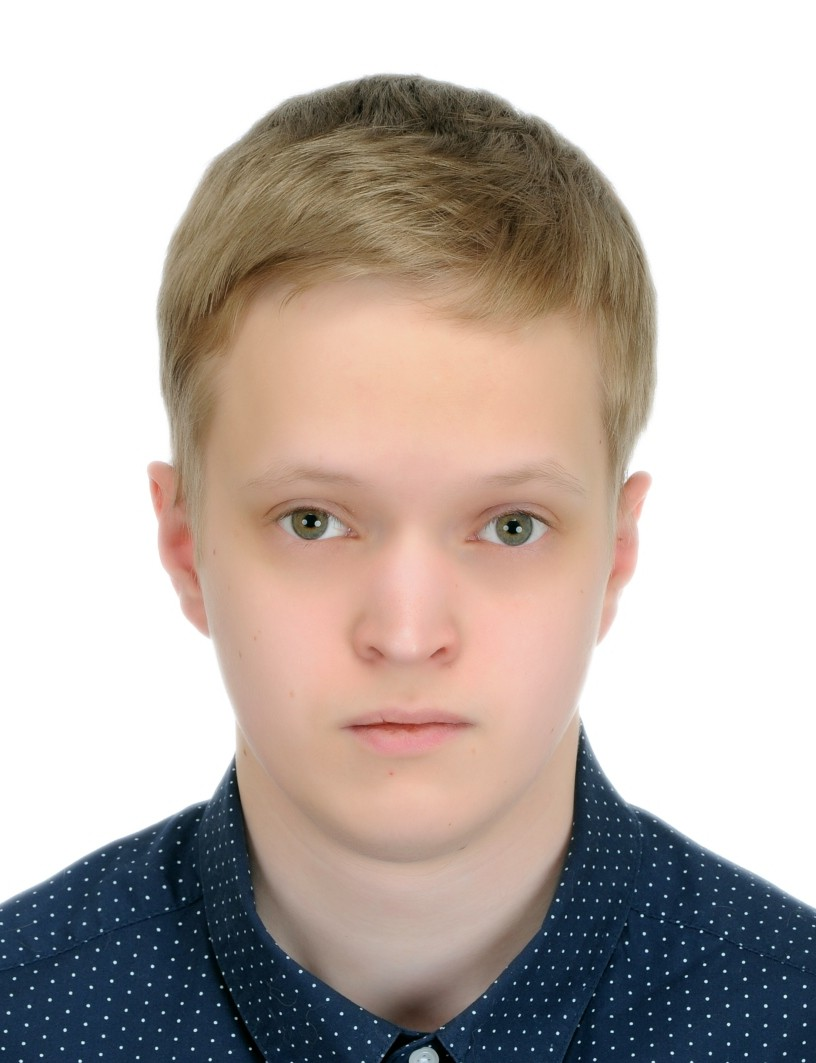
\includegraphics[keepaspectratio]{./image/Z.jpg}}
\end{column}
\end{columns}
\end{frame}

\section{Вводная
часть}\label{ux432ux432ux43eux434ux43dux430ux44f-ux447ux430ux441ux442ux44c}

\begin{frame}{Цель работы}
\protect\phantomsection\label{ux446ux435ux43bux44c-ux440ux430ux431ux43eux442ux44b}
\begin{itemize}[<+->]
\tightlist
\item
  Изучить три математические модели распространения рекламы.
\item
  Построить графики для заданных коэффициентов
\item
  Проанализировать влияние параметров
\item
  Найти момент максимальной скорости распространения рекламы
\end{itemize}

\#\# Модель Мальтуса

\textbf{Уравнение:} \[\frac{dn}{dt} = r\, n(t)\]

\begin{itemize}[<+->]
\tightlist
\item
  (n(t)) -- численность в момент (t)
\item
  (r\textgreater0) -- коэффициент роста
\end{itemize}

\textbf{Особенность:} неограниченный рост, без лимитирующих факторов

\textbf{Применение:} начальные этапы роста, демография, экономика
\end{frame}

\begin{frame}{Логистическая модель (рост с насыщением)}
\protect\phantomsection\label{ux43bux43eux433ux438ux441ux442ux438ux447ux435ux441ux43aux430ux44f-ux43cux43eux434ux435ux43bux44c-ux440ux43eux441ux442-ux441-ux43dux430ux441ux44bux449ux435ux43dux438ux435ux43c}
\textbf{Уравнение:}
\[\frac{dn}{dt} = r\, n(t)\left(1 - \frac{n(t)}{N}\right)\] или
\[\frac{dn}{dt} = \alpha\, n(t)\bigl(N - n(t)\bigr)\]

\begin{itemize}[<+->]
\tightlist
\item
  (N) -- «потолок» (ёмкость аудитории)
\item
  \textbf{Форма:} S-образная кривая, замедление при (n \to N)
\end{itemize}

\textbf{Применение:} биология, эпидемиология, маркетинг
\end{frame}

\begin{frame}{Модель распространения рекламы}
\protect\phantomsection\label{ux43cux43eux434ux435ux43bux44c-ux440ux430ux441ux43fux440ux43eux441ux442ux440ux430ux43dux435ux43dux438ux44f-ux440ux435ux43aux43bux430ux43cux44b}
\[\frac{dn}{dt} = \bigl(\alpha_1(t) + \alpha_2(t)\, n(t)\bigr)\bigl(N - n(t)\bigr)\]

\begin{itemize}[<+->]
\tightlist
\item
  (\alpha\_1(t)) -- \textbf{внешнее воздействие} (СМИ, листовки) -- не
  зависит от (n)
\item
  (\alpha\_2(t)) -- \textbf{внутреннее распространение} («сарафанное
  радио») -- зависит от числа знающих
\end{itemize}

\textbf{Влияние:} - (\alpha\_1) увеличивает скорость за счёт внешней
рекламы - (\alpha\_2) усиливает рост при больших (n) (каждый информирует
другого)
\end{frame}

\section{Выполнение лабораторной
работы}\label{ux432ux44bux43fux43eux43bux43dux435ux43dux438ux435-ux43bux430ux431ux43eux440ux430ux442ux43eux440ux43dux43eux439-ux440ux430ux431ux43eux442ux44b}

\begin{frame}{Постановка задачи}
\protect\phantomsection\label{ux43fux43eux441ux442ux430ux43dux43eux432ux43aux430-ux437ux430ux434ux430ux447ux438}
\textbf{Общие параметры:}

(N = 1224) (объём аудитории), (n(0) = 14)

\textbf{Три варианта модели:}

\begin{enumerate}[<+->]
\tightlist
\item
  (\displaystyle \frac{dn}{dt} = \bigl(0.61 + 0.000061, n\bigr)(N - n))
\item
  (\displaystyle \frac{dn}{dt} = \bigl(0.000073 + 0.73, n\bigr)(N - n))
\item
  (\displaystyle \frac{dn}{dt} = \bigl(0.7t + 0.6\cos(t), n\bigr)(N -
  n))
\end{enumerate}

\textbf{Задачи:} - Построить графики (n(t))
\end{frame}

\begin{frame}{Случай 1}
\protect\phantomsection\label{ux441ux43bux443ux447ux430ux439-1}
\[\alpha_1 = 0.61 \ (\text{велико}), \quad \alpha_2 = 6.1\cdot10^{-5} \ (\text{очень мало})\]

\begin{itemize}[<+->]
\tightlist
\item
  Рост почти полностью определяется внешним воздействием
\item
  Кривая быстро приближается к (N) \textbf{без S-образного изгиба}
\end{itemize}

\textbf{График:}\\
\pandocbounded{
\includegraphics[keepaspectratio]{image/1.png}}
\end{frame}

\begin{frame}{Случай 2}
\protect\phantomsection\label{ux441ux43bux443ux447ux430ux439-2}
\[\alpha_1 = 7.3\cdot10^{-5} \ (\text{пренебрежимо мало}), \quad \alpha_2 = 0.73\ \text{велико}\]

\begin{itemize}[<+->]
\tightlist
\item
  График моментально достигает плато
\item
  \textbf{Момент максимальной скорости} (по графику): (t \approx 0)
\end{itemize}

\pandocbounded{
\includegraphics[keepaspectratio]{image/2.png}}
\end{frame}

\begin{frame}{Случай 3}
\protect\phantomsection\label{ux441ux43bux443ux447ux430ux439-3}
\[\alpha_1(t) = 0.7t, \quad \alpha_2(t) = 0.6\cos(t)\]

\begin{itemize}[<+->]
\tightlist
\item
  График моментально достигает плато
\end{itemize}

\pandocbounded{
\includegraphics[keepaspectratio]{image/3.png}}
\end{frame}

\section{Выводы}\label{ux432ux44bux432ux43eux434ux44b}

\begin{frame}{Результаты}
\protect\phantomsection\label{ux440ux435ux437ux443ux43bux44cux442ux430ux442ux44b}
\begin{itemize}[<+->]
\tightlist
\item
  Изучены три модели динамики аудитории:

  \begin{itemize}[<+->]
  \tightlist
  \item
    Модель Мальтуса (неограниченный рост)
  \item
    Логистическая модель (S-образный рост с насыщением)
  \item
    Рекламная модель с двумя каналами воздействия
  \end{itemize}
\item
  Для заданных коэффициентов построены графики
\end{itemize}
\end{frame}




\end{document}
